% Collaboration flowchart — compact cheat-sheet variant.
% Shorter question wording, smaller font, narrower nodes.
\documentclass[tikz,border=4mm]{standalone}
\usepackage{tikz}
\usetikzlibrary{positioning, shapes.geometric, arrows.meta, calc}

\begin{document}
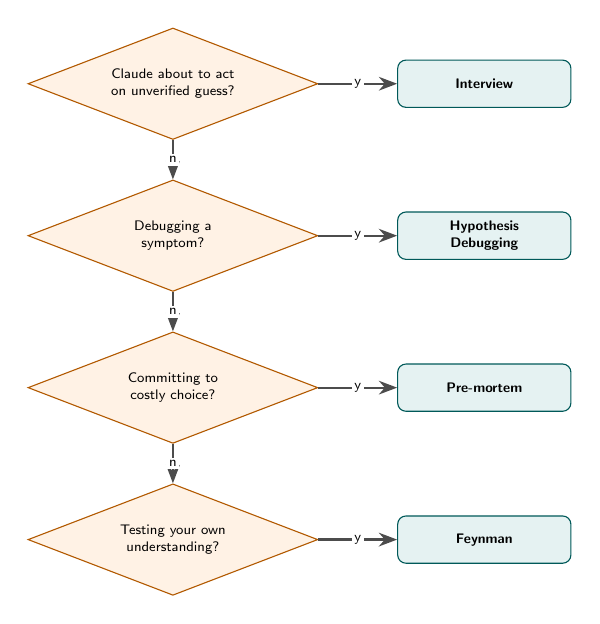
\begin{tikzpicture}[
  font=\sffamily,
  node distance=0.5cm and 1.0cm,
  question/.style={
    draw=orange!70!black, fill=orange!10, diamond, aspect=2.6,
    inner sep=0.5pt, align=center, text width=2.6cm, font=\sffamily\tiny
  },
  pattern/.style={
    draw=teal!70!black, fill=teal!10, rounded corners=3pt,
    minimum width=2.2cm, minimum height=0.6cm, align=center,
    font=\sffamily\tiny\bfseries
  },
  arrow/.style={-Stealth, thick, draw=gray!60!black},
  arrowlabel/.style={font=\sffamily\tiny, fill=white, inner sep=1pt},
]

\node[question] (q1) {Claude about to act \\ on unverified guess?};
\node[pattern, right=of q1] (interview) {Interview};

\node[question, below=of q1] (q2) {Debugging a \\ symptom?};
\node[pattern, right=of q2] (hyp) {Hypothesis \\ Debugging};

\node[question, below=of q2] (q3) {Committing to \\ costly choice?};
\node[pattern, right=of q3] (pre) {Pre-mortem};

\node[question, below=of q3] (q4) {Testing your own \\ understanding?};
\node[pattern, right=of q4] (feynman) {Feynman};

\draw[arrow] (q1) -- node[arrowlabel] {y} (interview);
\draw[arrow] (q1) -- node[arrowlabel] {n} (q2);
\draw[arrow] (q2) -- node[arrowlabel] {y} (hyp);
\draw[arrow] (q2) -- node[arrowlabel] {n} (q3);
\draw[arrow] (q3) -- node[arrowlabel] {y} (pre);
\draw[arrow] (q3) -- node[arrowlabel] {n} (q4);
\draw[arrow] (q4) -- node[arrowlabel] {y} (feynman);

\end{tikzpicture}
\end{document}
